\section{PID - 未完成(再包入第8章)}

所有PID控制器都是作用在误差信号$e(t)$上的。

\subsection{PID控制器}

\subsubsection{比例控制作用}

\begin{align*}
u(t)&=K_pe(t)\\
\frac{U(s)}{E(s)}&=K_p
\end{align*}

$K_p$称为比例增益。

\subsubsection{积分控制作用}

\begin{align*}
\frac{du(t)}{dt}&=K_ie(t)\\
u(t)&=K_i\int_0^te(t)dt\\
\frac{U(s)}{E(s)}&=\frac{K_i}{s}
\end{align*}

\subsubsection{比例+积分控制作用}

\begin{align*}
u(t)&=K_pe(t)+\frac{K_p}{T_i}\int_0^te(t)dt\\
\frac{U(s)}{E(s)}&=K_p\left(1+\frac{1}{T_is}\right)
\end{align*}

其中,$T_i$称为积分时间常数。

\subsubsection{比例+微分控制作用}

\begin{align*}
u(t)&=K_pe(t)+K_pT_d\frac{de(t)}{dt}\\
\frac{U(s)}{E(s)}&=K_p(1+T_ds)
\end{align*}

其中,$T_d$称为微分时间常数。

\subsubsection{比例+积分+微分控制作用}

\begin{align*}
u(t)&=K_pe(t)+\frac{K_p}{T_i}\int_0^te(t)dt+D_pT_d\frac{de(t)}{dt}\\
\frac{U(s)}{E(s)}&=K_p\left(1+\frac{1}{T_is}+T_ds\right)
\end{align*}

\subsection{积分和微分控制作用对系统性能的影响}

\subsubsection{积分控制作用}

如果传递函数中不存在积分器$1/s$,阶跃输入信号的响应一定会有稳态误差;通过引入积分控制系统,可以消除这种误差。

\subsubsection{比例控制}

对于阶跃输入信号,没有积分器时,一定存在稳态误差。

\begin{figure}[!ht]
	\centering
	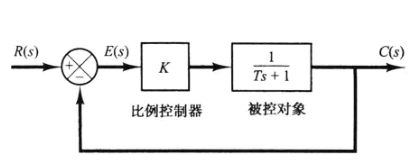
\includegraphics[width=8cm]{figures/13.png}
	\caption{比例控制系统}
	\label{13}
\end{figure}

如图\ref{13}所示的控制系统,

\begin{align*}
\frac{E(s)}{R(s)}&=\frac{R(s)-C(s)}{R(s)}=1-\frac{C(s)}{R(s)}=1-\frac{G(s)}{1+G(s)}=\frac{1}{1+G(s)}\\
E(s)&=\frac{1}{1+G(s)}R(s)=\frac{Ts+1}{Ts+1+K}\frac1s
\end{align*}

稳态误差为

\begin{equation*}
e_{ss}=\lim_{t\to\infty}e(t)=\lim_{s\to0}sE(s)=\lim_{s\to0}\frac{Ts+1}{Ts+1+K}=\frac{1}{K+1}
\end{equation*}

\subsubsection{积分控制}

积分控制可以消除稳态误差。如图\ref{14}所示的系统:

\begin{figure}[!ht]
	\centering
	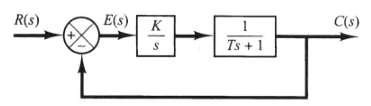
\includegraphics[width=8cm]{figures/14.png}
	\caption{积分控制系统}
	\label{14}
\end{figure}

\begin{align*}
\frac{C(s)}{R(s)}&=\frac{K}{s(Ts+1)+K}\\
{E(s)}&=\frac{s(Ts+1)}{s(Ts+1)+K}\frac1s
\end{align*}

稳态误差为

\begin{equation*}
e_{ss}=\lim_{t\to\infty}e(t)=\lim_{s\to0}sE(s)=\lim_{s\to0}\frac{s^2(Ts+1)}{Ts^2+s+K}\frac1s=0
\end{equation*}

\subsubsection{对转矩扰动的响应(比例控制)}

引入转矩扰动,如图\ref{15}所示,并令输入为$0$,即$R(s)=0$

\begin{figure}[!ht]
	\centering
	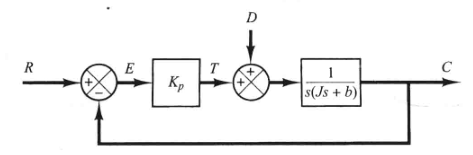
\includegraphics[width=8cm]{figures/15.png}
	\caption{转矩扰动(比例控制)}
	\label{15}
\end{figure}

考虑输出$C(s)$与扰动$D(s)$间的关系

\begin{equation*}
\frac{C(s)}{D(s)}=\frac{1}{Js^2+bs+K_p}
\end{equation*}

引起的误差

\begin{equation*}
\frac{E(s)}{D(s)}=\frac{R(s)-C(s)}{D(s)}=-\frac{1}{Js^2+bs+K_p}
\end{equation*}

假设扰动是一个幅值为$T_d$的阶跃扰动,$D(s)=T_d/s$,则稳态误差为

\begin{equation*}
e_{ss}=\lim_{t\to\infty}e(t)=\lim_{s\to0}sE(s)=\lim_{s\to0}\frac{-s}{Js^2+bs+K_p}\frac{T_d}{s}=-\frac{T_d}{K_p}
\end{equation*}

增大增益$K_p$可以减小稳态误差,但同时会导致系统响应的振荡加大。

\subsubsection{对转矩扰动的响应(比例+积分控制)}

在比例控制的基础上增加积分控制,可以消除稳态误差,如图\ref{16}所示:

\begin{figure}[!ht]
	\centering
	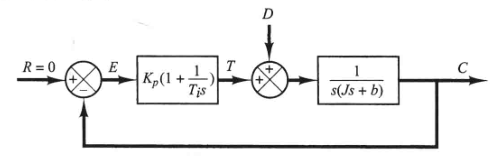
\includegraphics[width=8cm]{figures/16.png}
	\caption{转矩扰动(比例+积分控制)}
	\label{16}
\end{figure}

\begin{gather*}
\frac{C(s)}{D(s)}=\frac{s}{Js^3+bs^2+K_ps+\frac{K_p}{T_i}}\\
E(s)=-\frac{s}{Js^3+bs^2+K_ps+\frac{K_p}{T_i}}D(s)
\end{gather*}

如果特征方程

\begin{equation*}
Js^3+bs^2+K_ps+\frac{K_p}{T_i}=0
\end{equation*}

的根在左半平面,则系统稳定,稳态误差为

\begin{equation*}
e_{ss}=\lim_{t\to\infty}e(t)=\lim_{s\to0}sE(s)=\lim_{s\to0}\frac{-s^2}{Js^3+bs^2+K_ps+\frac{K_p}{T_i}}\frac{T_d}{s}=0
\end{equation*}

可以看出,稳态误差可以通过积分控制消除。在比例控制的基础上增加积分控制,会使二阶系统转变为三阶系统,如果$K_p$较大,特征方程的根需要注意保持在左半平面来保证系统稳定。

如果没有比例控制,仅靠积分控制,则系统总是不稳定的,因为特征方程$Js^3+bs^2+K=0$总有右半平面的根(韦达定理)。


\subsubsection{微分控制}

微分控制不能影响稳态误差,但是可以提前预知误差的变化,提前修正,增加系统阻尼,改善系统稳定性。

\subsubsection{惯性负载系统(比例控制)}

\begin{figure}[!ht]
	\centering
	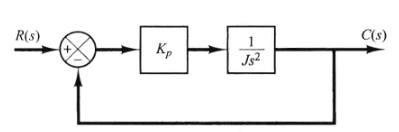
\includegraphics[width=8cm]{figures/17.png}
	\caption{惯性负载系统(比例控制)}
	\label{17}
\end{figure}

如图\ref{17}所示的惯性负载系统,其传递函数为:

\begin{equation*}
\frac{C(s)}{R(s)}=\frac{K_p}{Js^2+K_p}
\end{equation*}

特征方程:

\begin{equation*}
Js^2+K_p=0
\end{equation*}

显然方程有两个纯虚根,单位阶跃响应是无限期的持续振荡。

\subsubsection{惯性负载系统(比例+微分控制)}

\begin{figure}[!ht]
	\centering
	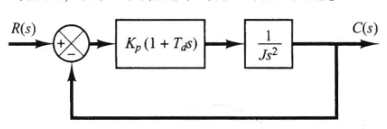
\includegraphics[width=8cm]{figures/18.png}
	\caption{惯性负载系统(比例+微分控制)}
	\label{18}
\end{figure}

如图\ref{18}所示,添加了微分控制,闭环传递函数为:

\begin{equation*}
\frac{C(s)}{R(s)}=\frac{K_p(1+T_ds)}{Js^2+K_pT_ds+K_p}
\end{equation*}

特征方程为:

\begin{equation*}
Js^2+K_pT_ds+K_p=0
\end{equation*}

特征方程的根都在左半平面,因此系统是稳定的。微分控制带来了阻尼效应。

\subsubsection{二级系统(比例+微分控制)}

\begin{figure}[!ht]
	\centering
	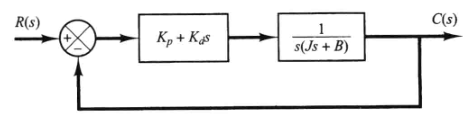
\includegraphics[width=8cm]{figures/19.png}
	\caption{二阶系统(比例+微分控制)}
	\label{19}
\end{figure}

如图\ref{19}所示的二阶系统,其闭环传递函数:

\begin{equation*}
\frac{C(s)}{R(s)}=\frac{K_p+K_ds}{Js^2+(B+K_d)s+K_p}
\end{equation*}

前文已经推导过,对于单位斜坡输入,其稳态误差为

\begin{equation*}
e_{ss}=\frac{B}{K_p}
\end{equation*}

阻尼比为

\begin{equation*}
\zeta=\frac{B+K_p}{2\sqrt{K_pJ}}
\end{equation*}

为了减小稳态误差,可以提高增益$K_p$、减小$B$,同时为了补偿阻尼比,减小振荡,还应同步地增大$K_d$,最终使阻尼比$\zeta$落在$0.4\sim0.7$的可以接受的范围内。




